\documentclass[10pt,a4paper]{article}

\usepackage[T1]{fontenc}
\usepackage[utf8]{inputenc}
\usepackage{lmodern}
\usepackage{microtype}
\usepackage[a4paper,margin=22mm]{geometry}
\usepackage{amsmath}
\usepackage{graphicx}
\usepackage{booktabs}
\usepackage{tabularx}
\usepackage{array}
\usepackage{multirow}
\usepackage{enumitem}
\usepackage{caption}
\usepackage[section]{placeins}
\usepackage[hidelinks]{hyperref}
\usepackage{xurl}

\setlength{\parindent}{0pt}
\setlength{\parskip}{0.38em}
\setlength{\tabcolsep}{4.2pt}
\renewcommand{\arraystretch}{1.12}
\setlist{nosep,leftmargin=1.45em}
\captionsetup{font=small}
\newcolumntype{Y}{>{\raggedright\arraybackslash}X}
\newcommand{\Rmodel}{\ensuremath{R_{\mathrm{model}}}}
\newcommand{\Rmax}{\ensuremath{R_{\mathrm{model}}^{\max}}}
\newcommand{\code}[1]{\texttt{#1}}

\title{Status Report Number 1}
\author{Thiago Mattar\\
\href{mailto:thiagocmattar@gmail.com}{\texttt{thiagocmattar@gmail.com}}}
\date{31 August 2026}

\hypersetup{
  pdftitle={Status Report Number 1},
  pdfauthor={Thiago Mattar}
}

\begin{document}
\maketitle

\section{Architecture and intervention ladder}

Figure~\ref{fig:ladder} locates the activation sites and organizes the progressive experimental program.

\begin{center}
  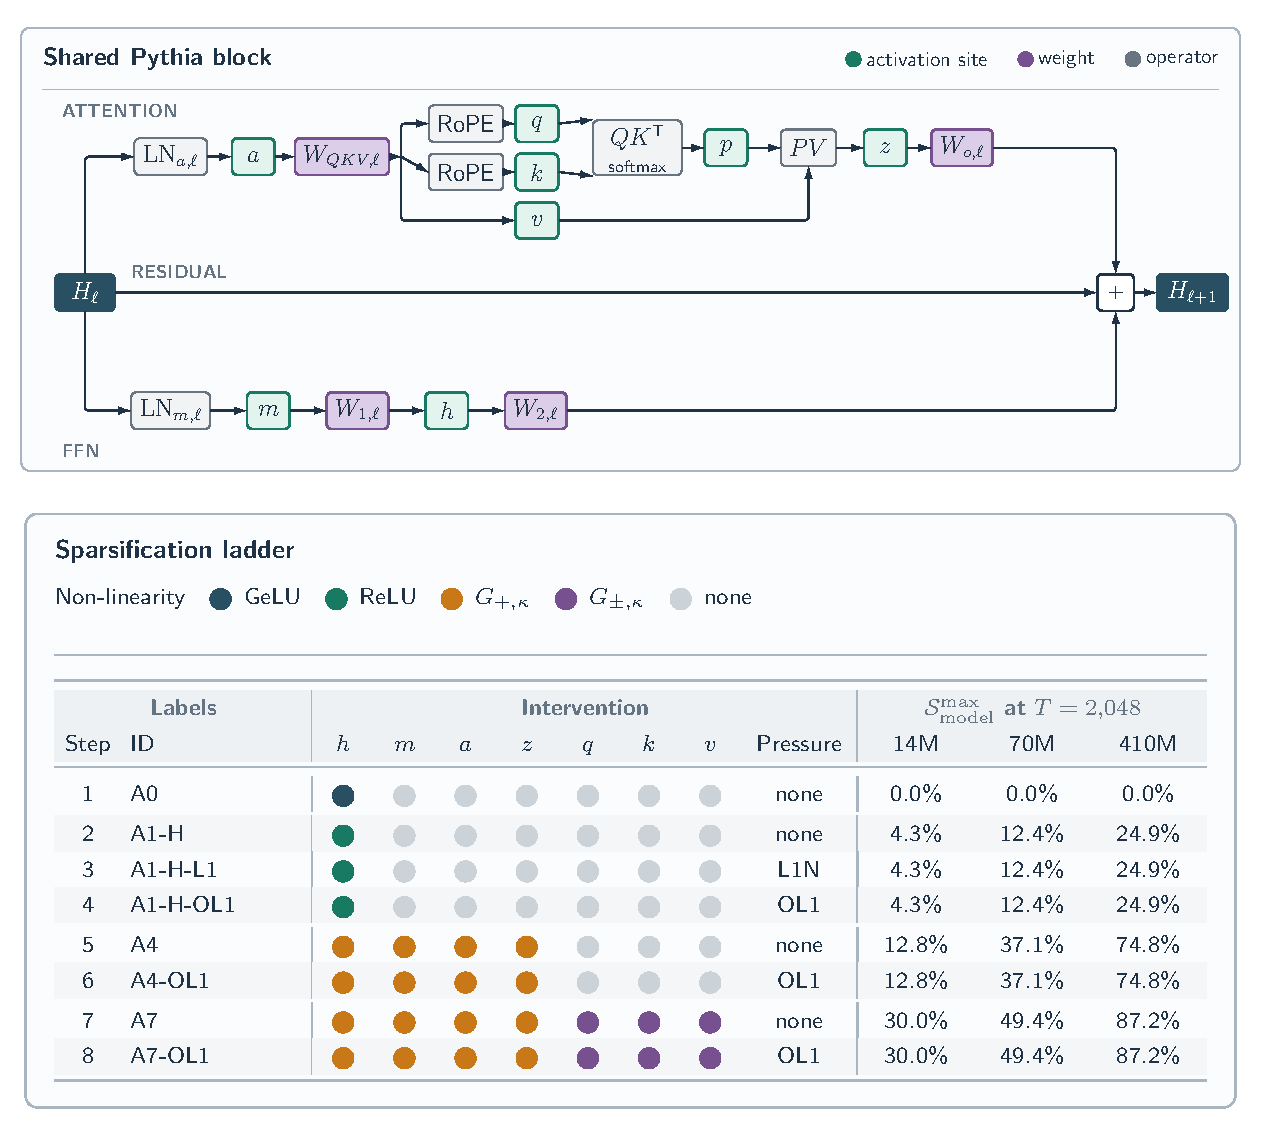
\includegraphics[width=0.80\textwidth]{../../artifacts/pythia-architecture-sparsification-ladder.pdf}
  \captionof{figure}{Shared Pythia block and sparsification intervention ladder. A4 and A7 denote operational topologies A4-Z and A7-Z-POST.}
  \label{fig:ladder}
\end{center}

\section{Experiment control}

\subsection{Scope dashboard}

\textbf{Pilot.} Local execution with 581 optimizer boundaries, global batch 64, and 76,152,832 training input tokens per condition.

\textbf{Paper-scale full pass.} RunPod A100 execution with 712 optimizer boundaries, global batch 1,024, and 1,493,172,224 training input tokens per condition. Conditions run concurrently across independent GPUs.

{\small
\begin{center}
\begin{minipage}{\textwidth}
\captionof{table}{Experiment scope at the report cutoff.}
\label{tab:scope}
\begin{tabularx}{\textwidth}{@{}l c Y c c@{}}
\toprule
\textbf{Step} & \textbf{Conditions/model} & \textbf{Pythia-14M} & \textbf{70M} & \textbf{410M} \\
\midrule
A0 & 1 & Full pass complete: Run 004 & 0/1 & 0/1 \\
A1-H & 1 & Full pass complete: Run 004 & 0/1 & 0/1 \\
A1-H-L1 & 4 & 4/4 full pass: Run 004 & 0/4 & 0/4 \\
A1-H-OL1 & 4 & 4/4 full pass: Run 009 & 0/4 & 0/4 \\
A4 & 5 & 5/5 full pass: Run 011 & 0/5 & 0/5 \\
A4-OL1 & 5 & 5/5 full pass: Run 015 & 0/5 & 0/5 \\
A7 & 5 & 5/5 full pass: Run 013 & 0/5 & 0/5 \\
A7-OL1 & 5 & 5/5 full pass: Run 014 & 0/5 & 0/5 \\
\bottomrule
\end{tabularx}
\end{minipage}
\end{center}}

\subsection{Paper-scale contract and parameter set}

The scale plan now adopts the size-specific learning rates in the standard Pythia recipe: peak/minimum $10^{-3}/10^{-4}$ for 14M and 70M, and $3\times10^{-4}/3\times10^{-5}$ for 410M. The study applies each activation intervention within this established recipe.

{\small
\begin{table}[htbp]
\centering
\caption{Shared paper-scale execution contract.}
\label{tab:contract}
\begin{tabularx}{\textwidth}{@{}p{37mm}Y@{}}
\toprule
\textbf{Field} & \textbf{Specification} \\
\midrule
Model construction & Random initialization from pinned Pythia architecture; model seed 1234 \\
Data & Pinned MiniPile cache; data-order seed 1234; sequence length 2,048 \\
Training horizon & 712 optimizer boundaries; 1,493,172,224 input tokens per condition \\
Global batch & 1,024 sequences; hardware-specific microbatch and accumulation preserve the product \\
Optimizer & AdamW, betas $(0.9,0.95)$, epsilon $10^{-8}$, weight decay 0.1, global clipping 1.0 \\
Schedule & 1\% linear warmup; cosine decay to 10\% of the size-specific peak learning rate \\
Precision & Dynamic FP16 autocast; FP32 parameters and optimizer state \\
Validation & 500 documents; 338 complete blocks; 692,224 input tokens; 1,444-token tail recorded \\
Retention & Activation counts and moments, weight norms, logical counts, pressure-gradient metrics, final checkpoint \\
\bottomrule
\end{tabularx}
\end{table}

\begin{table}[htbp]
\centering
\caption{Aggregated intervention parameter set. Threshold equality survives.}
\label{tab:parameters}
\begin{tabularx}{\textwidth}{@{}p{20mm}p{68mm}Y@{}}
\toprule
\textbf{Family} & \textbf{Gate and pressure} & \textbf{Parameter grid} \\
\midrule
A0 & Stock GeLU at \code{h} & Singleton \\
A1-H & ReLU at \code{h} & Singleton \\
A1-H-L1 & ReLU; naive L1 at \code{h} & $\lambda\in\{0.05,0.1,0.5,1.0\}$ \\
A1-H-OL1 & ReLU; OL1 at \code{h} & Same $\lambda$ grid; budget 1.0 \\
A4 & One-sided threshold at \code{a,m,h,z} & $\kappa\in\{0,0.01,0.05,0.1,0.5\}$ \\
A4-OL1 & A4 gates; OL1 at four sites & Same $\kappa$ grid; $\lambda=1$; budget 1.0 \\
A7 & A4 plus symmetric \code{q\_post,k\_post,v} gates & Same $\kappa$ grid \\
A7-OL1 & A7 gates; OL1 at seven sites & Same $\kappa$ grid; $\lambda=1$; budget 1.0 \\
\bottomrule
\end{tabularx}
\end{table}}

\section{RunPod compute}

Table~\ref{tab:runpod} reports elapsed wall-clock time for each condition's scientific process. Latest recorded RunPod cost across the six main-ladder runs is at least \$88.39; the retained 100 GB network volume remains separate at \$7/month.

{\small
\begin{center}
\begin{minipage}{\textwidth}
\captionof{table}{RunPod execution record. Wall-clock is elapsed scientific-process time per completed condition.}
\label{tab:runpod}
\setlength{\tabcolsep}{2.5pt}
\begin{tabularx}{\textwidth}{@{}p{12mm}p{62mm}Y r@{}}
\toprule
\textbf{Run} & \textbf{Compute} & \textbf{Wall-clock} & \textbf{Cost} \\
\midrule
004 & $5\times$ A100 80 GB; six conditions & 63--108 min & \$21.52 \\
009 & $4\times$ A100 80 GB; four conditions & 86--105 min & \$12.27 \\
011 & $5\times$ A100 80 GB; five conditions & 59--104 min & \$11.47 \\
015 & $5\times$ A100 80 GB; five conditions & 94--101 min & \$13.17* \\
013 & $5\times$ A100 80 GB; five conditions & 82--89 min & \$15.83 \\
014 & $5\times$ A100 80 GB; five conditions & 74--115 min & \$14.13 \\
\midrule
\textbf{Total} & \textbf{Latest recorded spend} & --- & \textbf{$\geq$\$88.39} \\
\bottomrule
\end{tabularx}
\end{minipage}
\end{center}}

*Run 015's \$13.17 is provisional because billing posting lagged teardown. Deployment required an 80 GB memory class, cache staging, detached execution, resumable artifact transfer, hash verification, and explicit teardown. The final Run 015 audit found zero Pods; the pre-existing retained volume was unchanged. Historical Run 012 compute and the combined spend including it are retained in Appendix~\ref{app:a4-ol1-h}.

\section{Results}

The analysis adds one intervention at each stage and maps the resulting validation-loss--logical-compute frontier. Only completed comparisons appear as result subsections.

All site columns report exact-zero percentages; \code{q} and \code{k} denote the post-RoPE tensors. ``n.m.'' denotes a site that was not measured in the source run.

{\small
\begin{table}[htbp]
\centering
\caption{Progressive analysis status.}
\label{tab:analysis-status}
\begin{tabularx}{\textwidth}{@{}c p{43mm}Y@{}}
\toprule
\textbf{Stage} & \textbf{Comparison} & \textbf{Evidence status} \\
\midrule
1 & A0 $\rightarrow$ A1-H & Full-pass endpoints complete \\
Control & A0/A1-H $\rightarrow$ uniform post-hoc clipping & Full-pass Analysis 005 complete \\
2 & A1-H $\rightarrow$ A1-H-L1 & Full-pass dose response complete \\
3 & A1-H-L1 $\rightarrow$ A1-H-OL1 & Matched full-pass Analysis 003 complete \\
4 & A1-H $\rightarrow$ A4 & Matched full-pass Analysis 004 complete \\
5 & A4 $\rightarrow$ A4-OL1 & Corrected Run 015 in Analysis 009; descriptive; F001 discarded \\
6 & A4 $\rightarrow$ A7 & Matched full-pass Analysis 008; tentative F002 \\
7 & A7 $\rightarrow$ A7-OL1 & Five matched full-pass pairs in Analysis 008; descriptive \\
\bottomrule
\end{tabularx}
\end{table}}
\FloatBarrier

\subsection{Type of non-linearity: A0 to A1-H}

ReLU creates a 63.448\% exact-zero rate at \code{h} and moves \Rmodel{} to 2.714\%.

{\small
\begin{table}[htbp]
\centering
\caption{Pythia-14M full-pass controls from Run 004.}
\setlength{\tabcolsep}{2.2pt}
\begin{tabular*}{\textwidth}{@{\extracolsep{\fill}}l*{9}{r}@{}}
\toprule
\textbf{Condition} & \textbf{Loss} & \textbf{\Rmodel{} (\%)} & \multicolumn{7}{c}{\textbf{Exact-zero (\%)}} \\
\cmidrule(l){4-10}
& & & \textbf{\code{h}} & \textbf{\code{m}} & \textbf{\code{a}} & \textbf{\code{z}} & \textbf{\code{q}} & \textbf{\code{k}} & \textbf{\code{v}} \\
\midrule
A0: GeLU & 5.209 & $<0.001$ & $<0.001$ & 0.000 & n.m. & n.m. & $<0.001$ & $<0.001$ & $<0.001$ \\
A1-H: ReLU & 5.270 & 2.714 & 63.448 & 0.000 & n.m. & n.m. & $<0.001$ & $<0.001$ & $<0.001$ \\
\bottomrule
\end{tabular*}
\end{table}}

The evaluation-only uniform TEAL-style control thresholds \code{a}, \code{m}, \code{h}, and \code{z} separately in every block; it does not threshold \code{q}, \code{k}, or \code{v}. For one common target $p$, values satisfying $|x|\leq t$ are zeroed without retraining. Table~\ref{tab:teal-controls} is the only result table that reports paired loss deltas.

{\small
\begin{table}[htbp]
\centering
\caption{Selected uniform TEAL-style post-hoc endpoints from \href{../../../analyses/005-2026-08-30-run004-controls-teal-posthoc/observations/O001-r-model-vs-final-validation-loss.md}{Analysis 005, Observation O001}. Deltas are paired to the independently evaluated $p=0$ row for the same checkpoint.}
\label{tab:teal-controls}
\setlength{\tabcolsep}{3.2pt}
\begin{tabular*}{\textwidth}{@{\extracolsep{\fill}}r*{6}{r}@{}}
\toprule
& \multicolumn{3}{c}{\textbf{GeLU control}} & \multicolumn{3}{c}{\textbf{ReLU control}} \\
\cmidrule(lr){2-4}\cmidrule(l){5-7}
$\boldsymbol{p}$ & \textbf{Loss} & $\boldsymbol{\Delta}$\textbf{loss} & \textbf{\Rmodel{} (\%)} & \textbf{Loss} & $\boldsymbol{\Delta}$\textbf{loss} & \textbf{\Rmodel{} (\%)} \\
\midrule
0.0 & 5.208594 & 0.000000 & $<0.001$ & 5.269633 & 0.000000 & 2.714133 \\
0.1 & 5.214453 & 0.005859 & 1.278706 & 5.274073 & 0.004439 & 3.568403 \\
0.2 & 5.250270 & 0.041676 & 2.554786 & 5.307940 & 0.038307 & 4.418365 \\
0.3 & 5.361901 & 0.153307 & 3.831641 & 5.405056 & 0.135422 & 5.271871 \\
0.4 & 5.605384 & 0.396790 & 5.125544 & 5.602965 & 0.333331 & 6.129325 \\
0.5 & 6.077731 & 0.869137 & 6.441923 & 5.976274 & 0.706641 & 6.994451 \\
\bottomrule
\end{tabular*}
\end{table}}
\FloatBarrier

\subsection{Naive L1 pressure: A1-H to A1-H-L1}

Increasing $\lambda$ raises exact-zero mass and \Rmodel{} across the four full-pass endpoints.

{\small
\begin{table}[htbp]
\centering
\caption{Run 004 full-pass naive-L1 dose response.}
\setlength{\tabcolsep}{2.2pt}
\begin{tabular*}{\textwidth}{@{\extracolsep{\fill}}r*{9}{r}@{}}
\toprule
$\boldsymbol{\lambda}$ & \textbf{Loss} & \textbf{\Rmodel{} (\%)} & \multicolumn{7}{c}{\textbf{Exact-zero (\%)}} \\
\cmidrule(l){4-10}
& & & \textbf{\code{h}} & \textbf{\code{m}} & \textbf{\code{a}} & \textbf{\code{z}} & \textbf{\code{q}} & \textbf{\code{k}} & \textbf{\code{v}} \\
\midrule
0.05 & 5.206 & 3.142 & 73.441 & 0.000 & n.m. & n.m. & $<0.001$ & $<0.001$ & $<0.001$ \\
0.10 & 5.165 & 3.336 & 77.993 & 0.000 & n.m. & n.m. & $<0.001$ & $<0.001$ & $<0.001$ \\
0.50 & 5.113 & 3.788 & 88.542 & 0.000 & n.m. & n.m. & $<0.001$ & $<0.001$ & $<0.001$ \\
1.00 & 5.102 & 3.949 & 92.323 & 0.000 & n.m. & n.m. & $<0.001$ & $<0.001$ & $<0.001$ \\
\bottomrule
\end{tabular*}
\end{table}}
\FloatBarrier

\subsection{Orthogonalization: A1-H-L1 to A1-H-OL1}

The matched full-pass endpoints occupy a narrow common region in validation loss, \Rmodel{}, and \code{h} sparsity.

{\small
\begin{table}[htbp]
\centering
\caption{Absolute naive-L1 and OL1 endpoints from Analysis 003.}
\label{tab:ol1-results}
\setlength{\tabcolsep}{2.0pt}
\begin{tabular*}{\textwidth}{@{\extracolsep{\fill}}rl*{9}{r}@{}}
\toprule
$\boldsymbol{\lambda}$ & \textbf{Method} & \textbf{Loss} & \textbf{\Rmodel{} (\%)} & \multicolumn{7}{c}{\textbf{Exact-zero (\%)}} \\
\cmidrule(l){5-11}
& & & & \textbf{\code{h}} & \textbf{\code{m}} & \textbf{\code{a}} & \textbf{\code{z}} & \textbf{\code{q}} & \textbf{\code{k}} & \textbf{\code{v}} \\
\midrule
\multirow{2}{*}{0.05} & L1  & 5.206 & 3.142 & 73.441 & 0.000 & n.m. & n.m. & $<0.001$ & $<0.001$ & $<0.001$ \\
                      & OL1 & 5.198 & 3.145 & 73.526 & 0.000 & n.m. & n.m. & $<0.001$ & $<0.001$ & $<0.001$ \\
\hline
\multirow{2}{*}{0.10} & L1  & 5.165 & 3.336 & 77.993 & 0.000 & n.m. & n.m. & $<0.001$ & $<0.001$ & $<0.001$ \\
                      & OL1 & 5.159 & 3.339 & 78.046 & 0.000 & n.m. & n.m. & $<0.001$ & $<0.001$ & $<0.001$ \\
\hline
\multirow{2}{*}{0.50} & L1  & 5.113 & 3.788 & 88.542 & 0.000 & n.m. & n.m. & $<0.001$ & $<0.001$ & $<0.001$ \\
                      & OL1 & 5.110 & 3.768 & 88.084 & 0.000 & n.m. & n.m. & $<0.001$ & $<0.001$ & $<0.001$ \\
\hline
\multirow{2}{*}{1.00} & L1  & 5.102 & 3.949 & 92.323 & 0.000 & n.m. & n.m. & $<0.001$ & $<0.001$ & $<0.001$ \\
                      & OL1 & 5.121 & 3.938 & 92.067 & 0.000 & n.m. & n.m. & $<0.001$ & $<0.001$ & $<0.001$ \\
\bottomrule
\end{tabular*}
\end{table}}

Figure~\ref{fig:ol1-projection} isolates the OL1 Adam-relative geometry before and after conflict projection.

\begin{figure}[htbp]
  \centering
  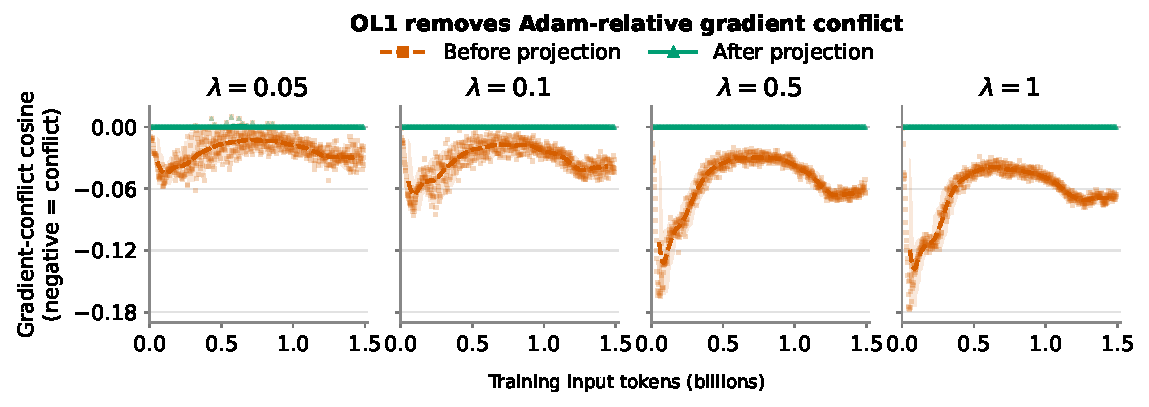
\includegraphics[width=0.84\textwidth]{../../../analyses/003-2026-08-30-run004-vs-run009-full-pass-l1-ol1/figures/03-ol1-orthogonalization-trajectories.pdf}
  \caption{OL1 Adam-relative interaction before and after conflict projection. Each panel contains 712 optimizer boundaries for one $\lambda$; lines are centered 51-boundary means and bands span p05--p95. Source: \href{../../../analyses/003-2026-08-30-run004-vs-run009-full-pass-l1-ol1/observations/O004-ol1-orthogonalization-trajectories.md}{Analysis 003, Observation O004}.}
  \label{fig:ol1-projection}
\end{figure}
\FloatBarrier

\subsection{Architecture-wide thresholding and OL1: A4 to A4-OL1}

A4 applies one-sided thresholds at \code{a}, \code{m}, \code{h}, and \code{z}. The corrected A4-OL1 objective in Run 015 adds post-gate OL1 pressure at all four sites with $\lambda=1$ and trust budget 1.0. It improves both validation loss and \Rmodel{} over matched A4 at $\kappa=0$ and $0.01$. At $\kappa=0.05$, $0.1$, and $0.5$, it adds 2.2506, 2.4413, and 2.4979 percentage points of \Rmodel{} for validation-loss costs of 0.055693, 0.128681, and 0.378307. This one-seed result remains descriptive; discarded Finding F001 is not restored.

{\small
\begin{table}[htbp]
\centering
\caption{Absolute A4 and corrected four-site A4-OL1 full-pass endpoints from \href{../../../analyses/009-2026-08-31-run012-vs-run015-a4-ol1-pressure-sites/observations/O001-h-only-vs-four-site-a4-ol1.md}{Analysis 009, Observation O001}. Every percentage is recomputed after pooling integer counts over all six layers and 338 complete validation blocks.}
\label{tab:a4-ol1-fullpass}
\setlength{\tabcolsep}{2.0pt}
\begin{tabular*}{\textwidth}{@{\extracolsep{\fill}}rl*{9}{r}@{}}
\toprule
$\boldsymbol{\kappa}$ & \textbf{Method} & \textbf{Loss} & \textbf{\Rmodel{} (\%)} & \multicolumn{7}{c}{\textbf{Exact-zero (\%)}} \\
\cmidrule(l){5-11}
& & & & \textbf{\code{h}} & \textbf{\code{m}} & \textbf{\code{a}} & \textbf{\code{z}} & \textbf{\code{q}} & \textbf{\code{k}} & \textbf{\code{v}} \\
\midrule
\multirow{2}{*}{0.00} & A4     & 5.470 & 7.212  & 68.765 & 49.779 & 48.560 & 54.525 & $<0.001$ & $<0.001$ & $<0.001$ \\
                      & A4-OL1 & 5.458 & 7.810  & 74.205 & 39.296 & 68.891 & 69.625 & $<0.001$ & $<0.001$ & $<0.001$ \\
\hline
\multirow{2}{*}{0.01} & A4     & 5.466 & 7.414  & 71.181 & 50.397 & 49.095 & 59.643 & $<0.001$ & $<0.001$ & $<0.001$ \\
                      & A4-OL1 & 5.458 & 8.587  & 80.833 & 43.464 & 73.491 & 85.259 & $<0.001$ & $<0.001$ & $<0.001$ \\
\hline
\multirow{2}{*}{0.05} & A4     & 5.434 & 8.206  & 81.340 & 52.712 & 51.155 & 77.641 & $<0.001$ & $<0.001$ & $<0.001$ \\
                      & A4-OL1 & 5.490 & 10.456 & 93.275 & 60.439 & 88.505 & 97.392 & $<0.001$ & $<0.001$ & $<0.001$ \\
\hline
\multirow{2}{*}{0.10} & A4     & 5.420 & 8.953  & 91.853 & 55.200 & 53.244 & 89.234 & $<0.001$ & $<0.001$ & $<0.001$ \\
                      & A4-OL1 & 5.548 & 11.394 & 97.149 & 75.912 & 91.310 & 99.283 & $<0.001$ & $<0.001$ & $<0.001$ \\
\hline
\multirow{2}{*}{0.50} & A4     & 5.660 & 10.216 & 99.876 & 66.386 & 63.434 & 99.881 & $<0.001$ & $<0.001$ & $<0.001$ \\
                      & A4-OL1 & 6.038 & 12.713 & 99.940 & 96.766 & 98.906 & 99.976 & $<0.001$ & $<0.001$ & 0.661 \\
\bottomrule
\end{tabular*}
\end{table}}
\FloatBarrier

\clearpage
\subsection{Attention-operand thresholding and OL1: A4 to A7 to A7-OL1}

A7 adds symmetric thresholds at post-RoPE \code{q}, \code{k}, and \code{v} to A4's one-sided \code{a}, \code{m}, \code{h}, and \code{z} gates; the matched A4/A7 result supports \href{../../../research/findings/F002-a7-extends-a4-logical-opportunity.md}{tentative Finding F002}. A7-OL1 adds post-gate orthogonal L1 pressure at all seven active sites with $\lambda=1$ and trust budget 1. At matched $\kappa=0.1$, A7-OL1 adds 1.3717 percentage points of \Rmodel{} for $+0.000816$ validation loss; at $\kappa=0.5$, it adds 12.0959 points for $+0.126466$ loss. The zero-threshold row regresses, so the A7/A7-OL1 effect is threshold-dependent and remains descriptive.

{\scriptsize
\begin{table}[htbp]
\centering
\caption{Matched A7 and A7-OL1 full-pass endpoints from \href{../../../analyses/008-2026-08-31-full-pass-frontier-with-a7/observations/O001-full-pass-frontier-with-a7.md}{Analysis 008, Observation O001}. Every percentage is recomputed after pooling integer counts over all six layers and 338 complete validation blocks. \code{out} is the ungated post-$W_o$ \code{attention\_output}.}
\label{tab:a7-a7-ol1-fullpass}
\setlength{\tabcolsep}{1.15pt}
\begin{tabular*}{\textwidth}{@{\extracolsep{\fill}}rl*{10}{r}@{}}
\toprule
$\boldsymbol{\kappa}$ & \textbf{Variant} & \textbf{Loss} & \textbf{\Rmodel{} (\%)} & \multicolumn{8}{c}{\textbf{Exact-zero mass (\%)}} \\
\cmidrule(l){5-12}
& & & & \textbf{\code{h}} & \textbf{\code{m}} & \textbf{\code{a}} & \textbf{\code{z}} & \textbf{\code{q}} & \textbf{\code{k}} & \textbf{\code{v}} & \textbf{\code{out}} \\
\midrule
\multirow{2}{*}{0.00} & A7     & 5.468401 & 7.217651  & 68.689 & 49.790 & 48.590 & 55.221 & $<0.001$ & $<0.001$ & $<0.001$ & $<0.001$ \\
                      & A7-OL1 & 5.480184 & 7.054229  & 68.277 & 49.503 & 48.583 & 42.761 & $<0.001$ & $<0.001$ & $<0.001$ & $<0.001$ \\
\hline
\multirow{2}{*}{0.01} & A7     & 5.458822 & 7.617649  & 71.275 & 50.330 & 49.064 & 59.041 & 0.399 & 0.407 & 1.654 & $<0.001$ \\
                      & A7-OL1 & 5.475797 & 7.723393  & 71.050 & 50.103 & 49.196 & 48.933 & 1.373 & 1.496 & 2.338 & $<0.001$ \\
\hline
\multirow{2}{*}{0.05} & A7     & 5.437888 & 9.126924  & 81.298 & 52.681 & 51.036 & 78.018 & 1.840 & 1.716 & 7.312 & $<0.001$ \\
                      & A7-OL1 & 5.462811 & 9.863032  & 81.052 & 52.241 & 51.036 & 72.067 & 5.427 & 5.817 & 10.526 & $<0.001$ \\
\hline
\multirow{2}{*}{0.10} & A7     & 5.428681 & 10.425018 & 91.353 & 55.075 & 53.052 & 90.052 & 3.150 & 3.227 & 11.355 & $<0.001$ \\
                      & A7-OL1 & 5.429497 & 11.796760 & 91.607 & 54.874 & 53.104 & 88.896 & 8.227 & 8.544 & 18.819 & $<0.001$ \\
\hline
\multirow{2}{*}{0.50} & A7     & 5.702923 & 15.386813 & 99.859 & 65.721 & 62.306 & 99.865 & 17.435 & 18.134 & 31.255 & $<0.001$ \\
                      & A7-OL1 & 5.829390 & 27.482684 & 99.876 & 68.698 & 75.732 & 99.918 & 93.545 & 94.541 & 98.713 & $<0.001$ \\
\bottomrule
\end{tabular*}
\end{table}}
\FloatBarrier

\subsection{Trained and post-hoc full-pass frontier}

Figure~\ref{fig:fullpass-frontier} places the trained endpoints and uniform TEAL-style clipping of the Run 004 controls on one validation-loss--\Rmodel{} plane. Its A4-OL1 series is the corrected four-site Run 015 result; historical Run 012 A4-OL1[\code{h}] is excluded from the main frontier and retained in Appendix~\ref{app:a4-ol1-h}. The figure also includes all five A7 and five A7-OL1 full-pass endpoints; Table~\ref{tab:a7-a7-ol1-fullpass} supplies their matched thresholds and count-pooled site values.

\begin{figure}[htbp]
  \centering
  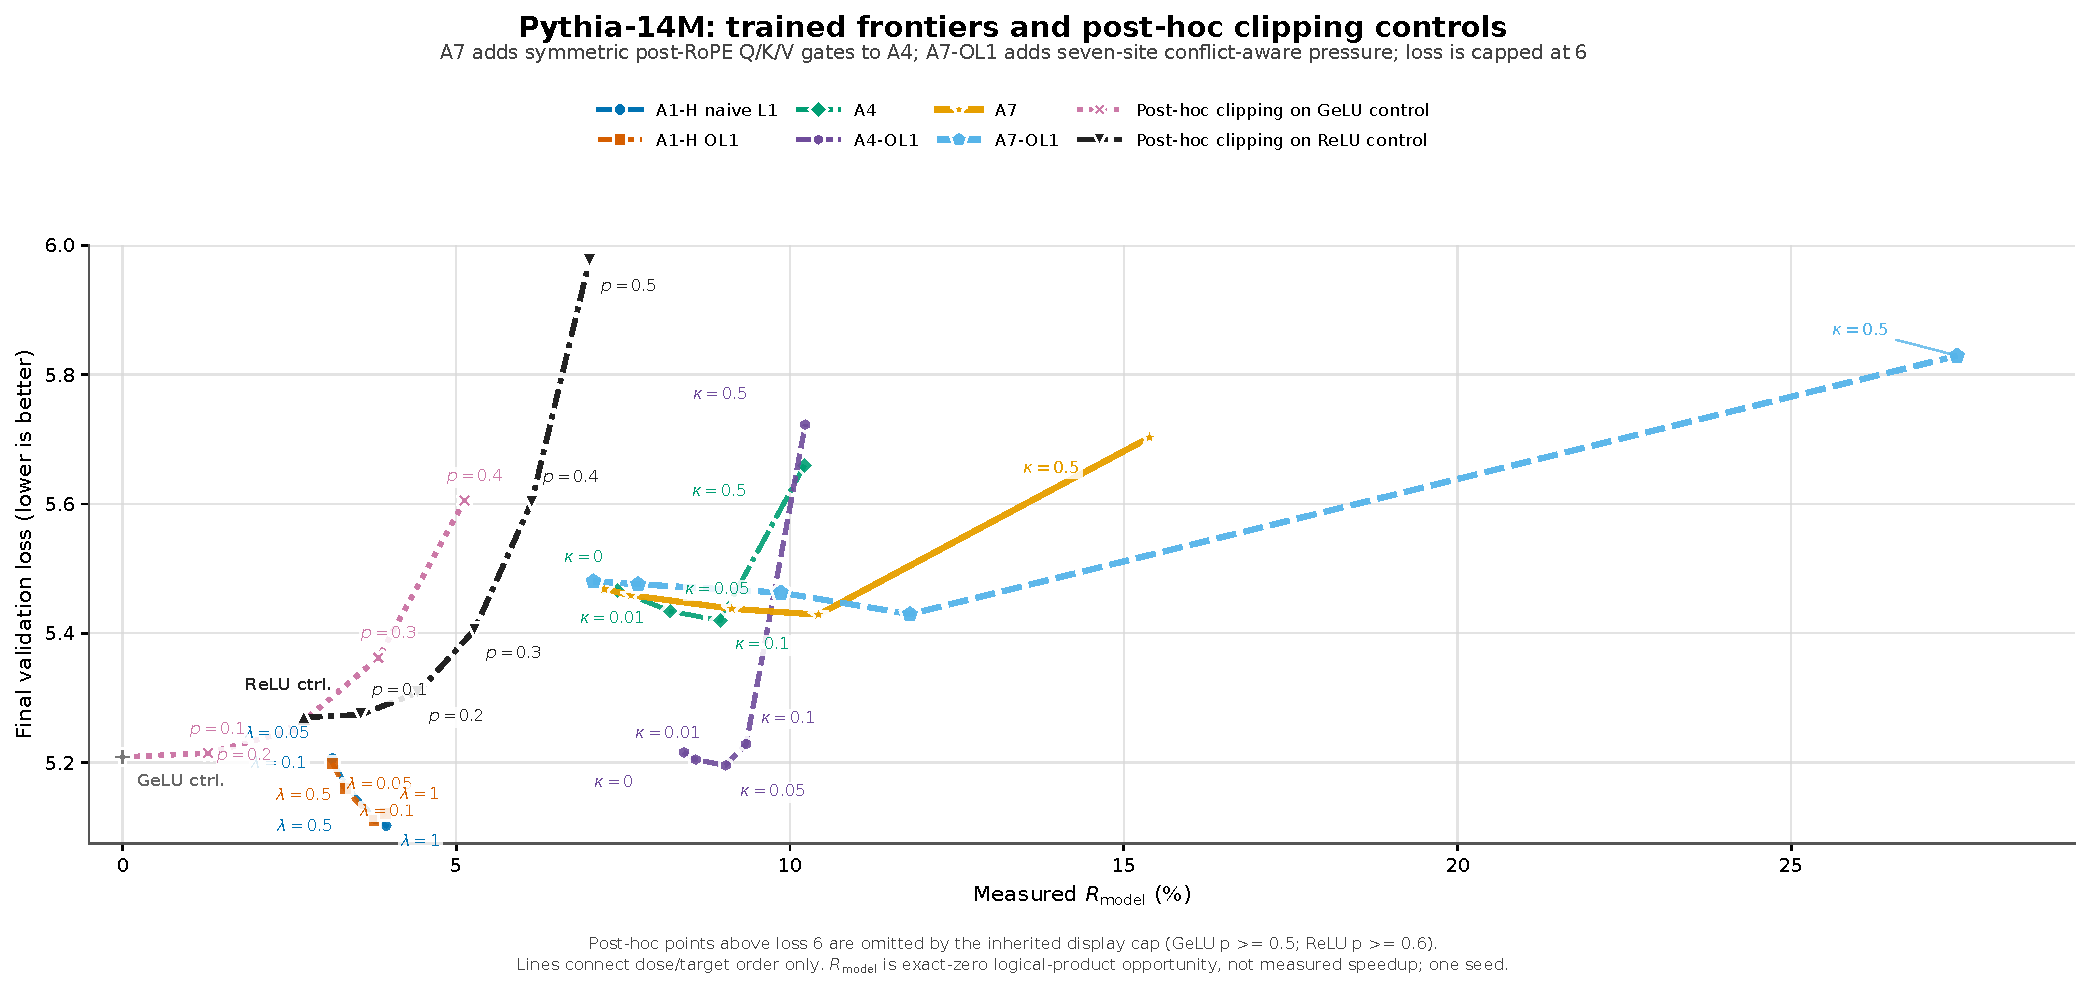
\includegraphics[width=0.92\textwidth]{../../../analyses/008-2026-08-31-full-pass-frontier-with-a7/figures/01-full-pass-frontier-with-a7.pdf}
  \caption{Corrected trained full-pass frontier, uniform TEAL-style post-hoc clipping of the Run 004 controls, Run 015 four-site A4-OL1, and the matched Run 013 A7 and Run 014 A7-OL1 endpoints. A7 uses one-sided thresholds at \code{a,m,h,z} and symmetric thresholds at post-RoPE \code{q,k,v}; A7-OL1 adds seven-site orthogonal L1 pressure. All trained endpoints are shown through loss 6.1; post-hoc points above loss 6 remain omitted by the inherited source filter. Lines indicate dose or target order only. Source: \href{../../../analyses/008-2026-08-31-full-pass-frontier-with-a7/observations/O001-full-pass-frontier-with-a7.md}{Analysis 008, Observation O001}.}
  \label{fig:fullpass-frontier}
\end{figure}

\appendix
\clearpage
\section{Historical A4-OL1[h] realization (Run 012)}
\label{app:a4-ol1-h}

Run 012 declared A4-OL1 pressure at \code{a,m,h,z}, but its frozen training code constructed the pressure capture with \code{["h"]}; the realized intervention was therefore A4 gates plus OL1 pressure only at \code{h}. The five endpoints remain valid for that realized A4-OL1[\code{h}] intervention, but they are excluded from the main four-site A4-OL1 result and cannot support discarded Finding F001.

{\small
\begin{table}[htbp]
\centering
\caption{Historical Run 012 A4-OL1[\code{h}] full-pass endpoints. Exact-zero percentages pool integer counts over all six layers and 338 complete validation blocks. Source: \href{../../../analyses/009-2026-08-31-run012-vs-run015-a4-ol1-pressure-sites/observations/O001-h-only-vs-four-site-a4-ol1.md}{Analysis 009, Observation O001}.}
\label{tab:a4-ol1-h-historical}
\setlength{\tabcolsep}{2.2pt}
\begin{tabular*}{\textwidth}{@{\extracolsep{\fill}}r*{9}{r}@{}}
\toprule
$\boldsymbol{\kappa}$ & \textbf{Loss} & \textbf{\Rmodel{} (\%)} & \multicolumn{7}{c}{\textbf{Exact-zero (\%)}} \\
\cmidrule(l){4-10}
& & & \textbf{\code{h}} & \textbf{\code{m}} & \textbf{\code{a}} & \textbf{\code{z}} & \textbf{\code{q}} & \textbf{\code{k}} & \textbf{\code{v}} \\
\midrule
0.00 & 5.216 & 8.409  & 93.543 & 49.816 & 49.413 & 64.671 & $<0.001$ & $<0.001$ & $<0.001$ \\
0.01 & 5.205 & 8.586  & 94.871 & 50.390 & 49.942 & 71.971 & $<0.001$ & $<0.001$ & $<0.001$ \\
0.05 & 5.196 & 9.036  & 97.915 & 52.391 & 51.791 & 88.307 & $<0.001$ & $<0.001$ & $<0.001$ \\
0.10 & 5.229 & 9.343  & 99.125 & 54.747 & 53.809 & 96.774 & $<0.001$ & $<0.001$ & $<0.001$ \\
0.50 & 5.723 & 10.227 & 99.944 & 66.441 & 63.622 & 99.934 & $<0.001$ & $<0.001$ & $<0.001$ \\
\bottomrule
\end{tabular*}
\end{table}}

\begin{figure}[htbp]
  \centering
  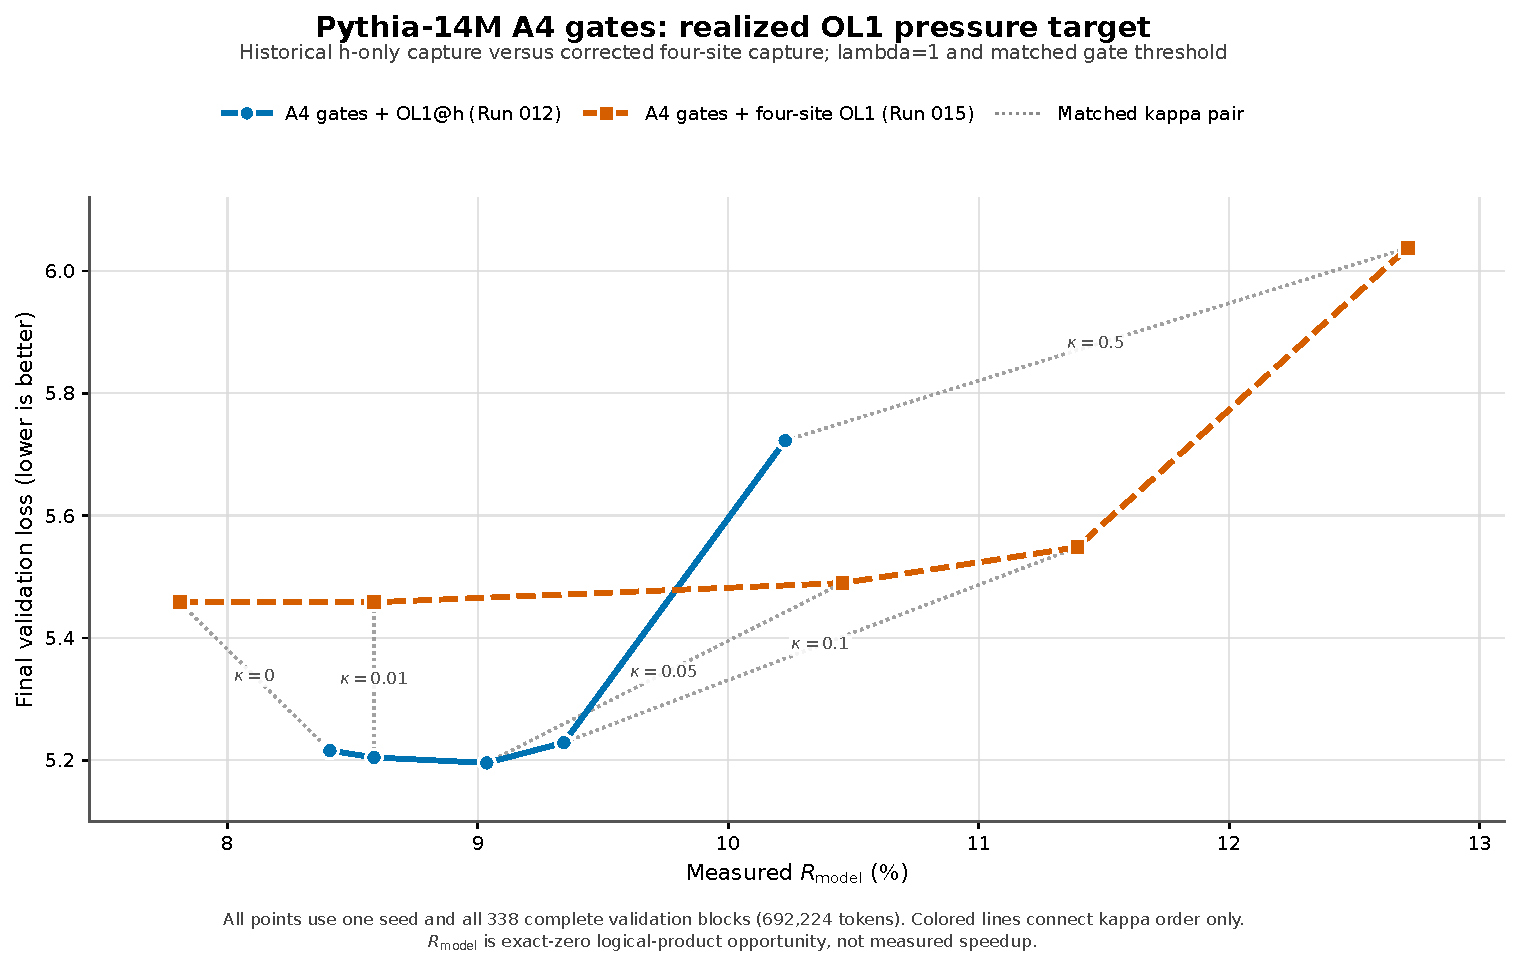
\includegraphics[width=0.92\textwidth]{../../../analyses/009-2026-08-31-run012-vs-run015-a4-ol1-pressure-sites/figures/01-rmodel-vs-validation-loss.pdf}
  \caption{Matched A4, historical Run 012 A4-OL1[\code{h}], and corrected Run 015 four-site A4-OL1. The historical and corrected pressure objectives are scientifically different interventions. Source: \href{../../../analyses/009-2026-08-31-run012-vs-run015-a4-ol1-pressure-sites/observations/O001-h-only-vs-four-site-a4-ol1.md}{Analysis 009, Observation O001}.}
  \label{fig:a4-ol1-h-appendix}
\end{figure}

Run 012 used five A100 80 GB Pods for 70--100 minutes per condition and cost \$14.77. Including this historical run, total recorded spend across the six main-ladder runs plus Run 012 is at least \$103.16; the Run 015 billing caveat stated in Section~3 still applies.

\end{document}
